\documentclass[UTF-8]{article}
\usepackage{amsmath}
\usepackage{amsthm}
\usepackage{amssymb}
\usepackage{graphicx}
\usepackage{geometry}
\usepackage{fancyhdr}
\usepackage{hyperref}
\usepackage{xcolor}
\usepackage{bm}
\usepackage{mathtools}


\title{FEM with Adjoint Method for Inverse Heat Conduction Problem}
\author{}
\date{}

\begin{document}
\maketitle

\section{An Iterative Finite-Element Algorithm for Solving Two-Dimensional Nonlinear Inverse Heat Conduction Problems}

\subsection{Primal Problem}
We have the primal problem which is the following system
\begin{equation}\label{equ001}
	\left\{
	\begin{array}{lll}
		\rho c(T) \frac{\partial T}{\partial t} = \nabla \cdot \left( \lambda (T) \nabla T \right) \quad &(\pmb{x},t) \in (\Omega, \mathcal{T}) &\text{(a)}\\
		T(\pmb{x},0) = \tilde{Y}^\xi & \pmb{x} \in \Omega &\text{(b)}\\
		\lambda(T) \nabla T \cdot \pmb{n} = q_u(\pmb{x},t) & (\pmb{x},t) \in (\Gamma_u, \mathcal{T}) &\text{(c)}\\
		\lambda(T) \nabla T \cdot \pmb{n} = q_g(\pmb{x},t) & (\pmb{x},t) \in (\Gamma_g, \mathcal{T}) &\text{(d)}
	\end{array}
	\right.
\end{equation}
In Eq.\ref{equ001}, $q_u$ is the unknown Neumann boundary condition on $\Gamma_u$ while $q_g$ is known on $\Gamma_g$.

\subsection{Objective Function}
From the primal problem, we define the objective function
\begin{equation}
	\mathcal{J}(q_{u}) = \frac{1}{2} \int_{0}^{t_f} \int_{\Gamma_g} \left(T-Y^\xi\right)^2 d\Gamma dt + \frac{\gamma}{2} \int_{0}^{t_f}\int_{\Gamma_u} \left(q_{u}\right)^2 d\Gamma dt.
\end{equation}

\subsection{Sensitivity Problem}
Next, we are going to derive the sensitivity problem. Firstly, we have the following definition
\begin{equation}
	\theta(\pmb{x},t;q_u,\Delta q_u) = \lim_{\epsilon \to 0} \frac{T(\pmb{x},t;q_u + \epsilon \Delta q_u) - T(\pmb{x},t;q_u)}{\epsilon},
\end{equation}
it is clear that
\begin{equation}\label{equ018}
	T(\pmb{x},t;q_u + \epsilon \Delta q_u) \approx T(\pmb{x},t;q_u) + \epsilon \theta(\pmb{x},t;q_u, \Delta q_u).
\end{equation}
For simplicity,
\begin{align*}
	&T^+ \coloneqq T(q_u + \epsilon \Delta q_u),\\
	&T \coloneqq T(q_u).
\end{align*}
From Eq.\ref{equ001}(a), we have
\begin{equation*}
	\rho c(T^+) \frac{\partial T^+}{\partial t} - \rho c(T) \frac{\partial T}{\partial t} = \nabla \left( \lambda(T^+) \nabla T^+ \right) - \nabla \left( \lambda(T) \nabla T \right).
\end{equation*}
Then
\begin{equation}\label{equ002}
	\rho c(T^+) \frac{\partial T}{\partial t} - \rho c(T) \frac{\partial T}{\partial t} + \epsilon \rho c(T^+) \frac{\partial \theta}{\partial t} = \nabla \left[ \left( \lambda (T^+) - \lambda(T) \right) \nabla T + \epsilon \lambda(T^+) \nabla \theta \right].
\end{equation}
Because of the next two equations
\begin{align}
	&\lim_{\epsilon \to 0} \frac{\rho c(T^+)-\rho c(T)}{\epsilon} = \frac{\partial \rho c}{\partial T} \theta, \\
	&\lim_{\epsilon \to 0} \frac{\lambda(T^+) - \lambda(T)}{\epsilon} = \frac{\partial \lambda}{\partial T} \theta,
\end{align}
divide $\epsilon$ on both sides of Eq.\ref{equ002} and let $\epsilon$ goes to $0$. We have
\begin{align}\label{equ003}
	\frac{\partial \rho c(T)}{\partial T} \theta \frac{\partial T}{\partial t} + \rho c(T) \frac{\partial \theta}{\partial t} &= \nabla \left[ \frac{\partial \lambda}{\partial T} \theta \nabla T + \lambda(T) \nabla \theta \right] \nonumber \\
	\frac{\rho c(T)}{\partial t} \theta + \rho c(T) \frac{\partial \theta}{\partial t} &= \nabla \left( \theta \frac{\partial \lambda}{\partial T} \nabla T \right) + \nabla \lambda(T) \nabla \theta \nonumber \\
	\frac{\partial \rho c(T) \theta}{\partial t} &= \nabla^2 \left( \lambda(T) \theta \right).
\end{align}

Next, from Eq.\ref{equ001}(b), we have
\begin{align*}
	T^+(\pmb{x},0) &= Y^\xi\\
	T(\pmb{x},0) &= Y^\xi.
\end{align*}
It is easy to get
\begin{equation}\label{equ004}
	\theta(\pmb{x},0) = 0.
\end{equation}

At last, we will derive the boundary conditions of the sensitivity problem. From Eq.\ref{equ001}(c), we can get
\begin{align*}
	\lambda(T^+) \nabla T^+ \cdot \pmb{n} &= q_u + \epsilon \Delta q_u,\\
	\lambda(T) \nabla T \cdot \pmb{n} &= q_u.
\end{align*}
Subtract them and we have
\begin{align*}
	\left[ \lambda (T^+) \nabla T^+ - \lambda(T) \nabla T \right] \cdot \pmb{n} &= \epsilon \Delta q_u\\
	\left[ \lambda (T^+) \nabla T + \lambda (T^+) \epsilon \nabla \theta - \lambda(T) \nabla T \right] \cdot \pmb{n} = \epsilon \Delta q_u.
\end{align*}
Divide $\epsilon$ on both sides of the equation above and let $\epsilon$ goes to $0$. Then, we have
\begin{align}\label{equ005}
	\left[ \frac{\partial \lambda}{\partial T} \theta \nabla T + \lambda(T) \nabla \theta \right] \cdot \pmb{n} &= \Delta q_u \nonumber \\
	\nabla\left( \lambda(T) \theta \right) \cdot \pmb{n} &= \Delta q_u.
\end{align}
Notice that, Eq.\ref{equ005} is satisfied on boundary $\Gamma_u$.

Similarly, we can also get
\begin{equation}\label{equ006}
	\nabla \left( \lambda(T) \theta \right) \cdot \pmb{n} = 0
\end{equation}
on boundary $\Gamma_g$.

With Eq.\ref{equ003}, Eq.\ref{equ004}, Eq.\ref{equ005} and Eq.\ref{equ006}, we can define the sensitivity problem
\begin{equation}\label{equ007}
	\left\{
	\begin{array}{lll}
		\rho \frac{\partial \left( c(T) \theta \right)}{\partial t} = \nabla^2 \left( \lambda(T) \theta \right) \quad &(\pmb{x},t) \in (\Omega,\mathcal{T}) &(a)\\
		\theta(\pmb{x},t;q_u,\Delta q_u) = 0 &\pmb{x}\in \Omega &(b)\\
		\nabla\left( \lambda(T) \theta \right) \cdot \pmb{n} = \Delta q_u(\pmb{x},t) &(\pmb{x},t) \in (\Gamma_u, \mathcal{T}) &(c)\\
		\nabla\left( \lambda(T) \theta \right) \cdot \pmb{n} = 0 &(\pmb{x},t) \in (\Gamma_g, \mathcal{T}) &(d)\\		
	\end{array}
	\right.
\end{equation}

\subsection{Dual Problem}
Now, let's derive the dual problem. From Eq.\ref{equ007}(a), we can get
\begin{equation*}
	\rho \frac{\partial \left( c(T) \theta \right)}{\partial t} - \nabla^2 \left( \lambda(T) \theta \right) = 0.
\end{equation*}
Multiply both sides of the equation above by $\phi$ and integrate on spatial domain $\Omega$ and time domain $\mathcal{T}$
\begin{align}\label{equ020}
	0 =& \int_{0}^{t_f} \int_\Omega \left[ \rho \frac{\partial \left(c(T)\theta\right)}{\partial t} - \nabla^2\left( \lambda(T) \theta \right) \right] \phi d\Omega dt \nonumber \\
	=& \int_\Omega \int_{0}^{t_f} \rho \phi d\left( c(T)\theta \right) d\Omega - \int_{0}^{t_f} \int_{\partial \Omega} \nabla\left( \lambda(T)\theta \right) \cdot \pmb{n} \phi d\Gamma dt + \int_{0}^{t_f} \int_\Omega \nabla\left( \lambda(T)\theta \right) \nabla\phi d\Omega dt \nonumber \\
	=& \int_\Omega  \rho \phi c(T)\theta \big|_0^{t_f} d\Omega - \int_{0}^{t_f} \int_\Omega \rho c(T) \theta \frac{\partial \phi}{\partial t} d\Omega dt - \int_{0}^{t_f} \int_{\partial \Omega} \nabla\left( \lambda(T)\theta \right) \cdot \pmb{n} \phi d\Gamma dt + \int_{0}^{t_f} \int_\Omega \nabla\left( \lambda(T)\theta \right) \nabla\phi d\Omega dt \nonumber \\
	=& \int_\Omega  \rho \phi c(T)\theta \big|_{t_f} d\Omega - \int_{0}^{t_f} \int_{\Gamma_u} \nabla\left( \lambda(T)\theta \right) \cdot \pmb{n} \phi d\Gamma dt + \int_{0}^{t_f} \int_\Omega \nabla\left( \lambda(T)\theta \right) \nabla\phi d\Omega dt - \int_{0}^{t_f} \int_\Omega \rho c(T) \theta \frac{\partial \phi}{\partial t} d\Omega dt \nonumber \\
	=& \int_\Omega  \rho \phi c(T)\theta \big|_{t_f} d\Omega - \int_{0}^{t_f} \int_{\Gamma_u} \nabla\left( \lambda(T)\theta \right) \cdot \pmb{n} \phi d\Gamma dt - \int_{0}^{t_f} \int_\Omega \nabla^2 \phi \left( \lambda(T)\theta \right) d\Omega dt \nonumber \\
	&+ \int_{0}^{t_f} \int_{\partial \Omega} \nabla\phi\cdot \pmb{n} \left( \lambda(T)\theta \right) d\Omega dt - \int_{0}^{t_f} \int_\Omega \rho c(T) \theta \frac{\partial \phi}{\partial t} d\Omega dt \nonumber \\
	=& \int_\Omega  \rho c(T)\theta \phi \big|_{t_f} d\Omega - \int_{0}^{t_f} \int_{\Gamma_u} \Delta q_u \phi d\Gamma dt - \int_{0}^{t_f} \int_\Omega \left[ \rho c(T) \frac{\partial \phi}{\partial t} + \lambda(T) \nabla^2 \phi \right] \theta d\Omega dt \nonumber \\
	&+ \int_{0}^{t_f} \int_{\Gamma_u} \lambda(T) \nabla\phi\cdot \pmb{n} \theta  d\Omega dt + \int_{0}^{t_f} \int_{\Gamma_g} \lambda(T) \nabla\phi\cdot \pmb{n} \theta d\Omega dt.
\end{align}

From the definition of Eq.\ref{equ001}, we can get
\begin{align}
	\mathcal{J}(q_u + \epsilon \Delta q_u) - \mathcal{J}(q_u) = &\frac{1}{2} \int_{0}^{t_f} \int_{\Gamma_g} \left(T + \epsilon \theta - Y^\xi \right)^2 d\Gamma dt + \frac{\gamma}{2} \int_{0}^{t_f}\int_{\Gamma_u} \left(q_u + \epsilon \Delta q_u \right)^2 d\Gamma dt \nonumber \\
	&- \frac{1}{2} \int_{0}^{t_f} \int_{\Gamma_g} \left(T - Y^\xi \right)^2 d\Gamma dt - \frac{\gamma}{2} \int_{0}^{t_f}\int_{\Gamma_u} \left( q_u \right)^2 d\Gamma dt \nonumber \\
	=& \frac{1}{2} \int_{0}^{t_f} \int_{\Gamma_g} \left( 2 \epsilon \theta T - 2 \epsilon \theta Y^\xi + \epsilon^2 \theta^2  \right) d\Gamma dt + \frac{\gamma}{2} \int_{0}^{t_f} \int_{\Gamma_u} \left( 2\epsilon q_u \Delta q_u + \epsilon^2 \Delta q_u^2 \right)d \Gamma dt \nonumber 
\end{align}
Then
\begin{align}\label{equ013}
	\left(\mathcal{J}(q_u),\Delta q_u \right) =& \lim_{\epsilon \to 0} \frac{\mathcal{J}(q_u + \epsilon \Delta q_u) - \mathcal{J}(q_u)}{\epsilon} \nonumber \\
	=& \int_{0}^{t_f} \int_{\Gamma_g} \theta \left( T - Y^\xi \right) d\Gamma dt + \gamma \int_{0}^{t_f} \int_{\Gamma_u} q_u \Delta q_u d\Gamma dt
\end{align}

Based on Eq.\ref{equ013} and Eq.\ref{equ020}, we can get the dual problem

\begin{equation}\label{equ008}
	\left\{
	\begin{array}{lll}
		\rho c(T) \frac{\partial \phi}{\partial t} = -\lambda(T) \nabla^2 \phi \quad &(\pmb{x},t) \in (\Omega,\mathcal{T}) &(a) \\
		\phi(\pmb{x},t_{\text{max}}) = 0 &\pmb{x} \in \Omega &(b)\\
		\lambda(T) \nabla\phi \cdot \pmb{n} = 0 &(\pmb{x},t) \in (\Gamma_u, \mathcal{T}) &(c)\\
		\lambda(T) \nabla\phi \cdot \pmb{n} = T(\pmb{x},t;q_u) - Y^\xi &(\pmb{x},t) \in (\Gamma_g, \mathcal{T}) &(d)\\
	\end{array}
	\right.
\end{equation}


\subsection{Derivative of Objective Function}
Multiply both sides of Eq.\ref{equ007}(a) by $\phi$ and integrate on $\Omega$
\begin{equation}\label{equ009}
	\int_{0}^{t_f} \int_\Omega \rho \frac{\partial \left( c(T) \theta \right)}{\partial t} \phi d\Gamma dt = \int_0^{t_f} \int_\Omega \nabla \cdot \nabla \left( \lambda(T) \theta \right) \phi d\Gamma dt.
\end{equation}
Left hand side of Eq.\ref{equ009} is
\begin{align}\label{equ010}
	LHS =& \int_\Omega \int_0^{t_f} \rho \phi d\left(c(T)\right) d\Omega \nonumber \\
	=& \int_\Omega \left[ \rho \phi c(T) \theta \Big|_0^{t_f} - \int_{0}^{t_f} \rho c(T) \theta \frac{\partial \phi}{\partial t} dt \right] d\Omega \nonumber \\
	=& \int_\Omega \int_{0}^{t_f} \lambda(T) \nabla^2\phi \theta dt d\Omega \nonumber \\
	=& \int_0^{t_f}\int_{\partial \Omega} \lambda(T) \nabla\phi \cdot \pmb{n} \theta d\Gamma dt - \int_{0}^{t_f} \int_\Omega \nabla \left( \lambda(T) \theta \right) \nabla \phi d\Omega dt \nonumber \\
	=& \int_0^{t_f}\int_{\Gamma_g} \lambda(T) \nabla\phi \cdot \pmb{n} \theta d\Gamma dt - \int_{0}^{t_f} \int_\Omega \nabla \left( \lambda(T) \theta \right) \nabla \phi d\Omega dt.
\end{align}
In Eq.\ref{equ010}, the third equality comes from Eq.\ref{equ007}(b) and Eq.\ref{equ008}(b) and the last equality comes from Eq.\ref{equ008}(c). Right hand side of Eq.\ref{equ009} is
\begin{align}\label{equ011}
	RHS =& \int_{0}^{t_f} \int_{\partial \Omega} \nabla \left( \lambda(T) \theta \right) \cdot \pmb{n} \phi d\Omega dt - \int_{0}^{t_f} \int_\Omega \nabla \left( \lambda(T) \theta \right) \nabla \phi d\Omega dt \nonumber \\
	=& \int_{0}^{t_f} \int_{\Gamma_u} \nabla \left( \lambda(T) \theta \right) \cdot \pmb{n} \phi d\Omega dt - \int_{0}^{t_f} \int_\Omega \nabla \left( \lambda(T) \theta \right) \nabla \phi d\Omega dt
\end{align}
The second equality of Eq.\ref{equ011} comes from Eq.\ref{equ007}(d). Combine Eq.\ref{equ010} and Eq.\ref{equ011}, we can get
\begin{equation*}
	\int_{0}^{t_f}\int_{\Gamma_g} \lambda(T) \nabla\phi \cdot \pmb{n} \theta d\Omega dt = \int_{0}^{t_f} \int_{\Gamma_u} \nabla\left( \lambda(T) \theta \right) \cdot \pmb{n} \phi d\Omega dt.
\end{equation*}
With Eq.\ref{equ007}(c) and Eq.\ref{equ008}(d), the equation above becomes
\begin{equation}\label{equ012}
	\int_{0}^{t_f} \int_{\Gamma_g} \left( T-Y^\xi \right) \theta d\Omega dt = \int_{0}^{t_f} \int_{\Gamma_u} \Delta q_u \phi d\Omega dt.
\end{equation}
Combining Eq.\ref{equ013} and Eq.\ref{equ012}, here comes
\begin{align}\label{equ014}
		\left(\mathcal{J}(q_u),\Delta q_u \right) =& \int_{0}^{t_f} \int_{\Gamma_g} \theta \left( T - Y^\xi \right) d\Gamma dt + \gamma \int_{0}^{t_f} \int_{\Gamma_u} q_u \Delta q_u d\Gamma dt \nonumber \\
	=& \int_{0}^{t_f} \int_{\Gamma_u} \phi \Delta q_u d\Gamma dt + \gamma \int_{0}^{t_f} \int_{\Gamma_u} q_u \Delta q_u d\Gamma dt \nonumber \\
	=& \int_{0}^{t_f} \int_{\Gamma_u} \left( \phi + \gamma q_u \right) \Delta q_u d\Gamma dt.
\end{align}
So it proves that Eq.\ref{equ016}
\begin{equation}\label{equ016}
	\mathcal{J}^\prime (q_{u}) = \phi + \gamma q_{u}.
\end{equation}

\subsection{Optimal Step Size}
The expression for the optimal step size $\alpha_k$ is
\begin{equation}\label{equ017}
	\alpha_k = -\frac{\int_{0}^{t_f} \int_{\Gamma_g} \left(T_k - Y^\xi\right) \theta_k d\Gamma dt + \gamma_{k+1} \int_{0}^{t_f} \int_{\Gamma_u} \Delta q_{u,k} q_{u,k} d\Gamma dt }{\int_{0}^{t_f} \int_{\Gamma_g} \theta_k^2 d\Gamma dt + \gamma_{k+1} \int_{0}^{t_f} \int_{\Gamma_u} \Delta q_{u,k}^2 d\Gamma dt }.
\end{equation}

In Eq.\ref{equ018}, we replace $\epsilon$ with $\alpha$, then
\begin{align*}
	\mathcal{J}(q_{u,k+1}) =& \mathcal{J}(q_{u,k} + \alpha_k \Delta q_{u,k}) \nonumber \\
	=& \frac{1}{2} \int_{0}^{t_f} \int_{\Gamma_g} (T_{k+1} - Y^\xi)^2 d\Gamma dt + \frac{\gamma_{k+1}}{2} \int_{0}^{t_f} \int_{\Gamma_u} (q_{u,k+1})^2 d\Gamma dt \nonumber \\
	=& \frac{1}{2} \int_{0}^{t_f} T_k^2 + \alpha_k^2 \theta_k^2 + (Y^\xi)^2 - 2T_k Y^\xi - 2 \alpha_k \theta_k Y^\xi + 2 T_k \alpha_k \theta_k d\Gamma dt \nonumber \\
	& + \frac{\gamma_{k+1}}{2} \int_{0}^{t_f} \int_{\Gamma_u} q_{u,k}^2 + \alpha_k^2 \Delta q_{u,k}^2 + 2 \alpha _k q_{u,k} \Delta q_{u,k} d\Gamma dt
\end{align*}
Taking derivative of $\mathcal{J}(q_{u,k+1})$ with $\alpha_k$, we have
\begin{equation}\label{equ019}
	\frac{\partial \mathcal{J}(q_{u,k+1})}{\partial \alpha_k} = \int_{0}^{t_f}\int_{\Gamma_g} \alpha_k \theta_k^2 - \theta_k Y^\xi + \theta_k T_k d\Gamma dt + \gamma_{k+1} \int_{0}^{t_f} \int_{\Gamma_u} \alpha_k \Delta q_{u,k}^2 + q_{u,k} \Delta q_{u,k} d\Gamma dt.
\end{equation}
Let Eq.\ref{equ019} equals to $0$ and we can get Eq.\ref{equ017}.

\section{FEM with Adjoint Method for Solving Multi-layers Inverse Heat Conduction Problem}

\subsection{Primal Problem}
We study on a multi-layers inverse heat condution problem which is defined on the domain showed in Fig.\ref{fig001}. 
\begin{figure}[ht]
	\centering
	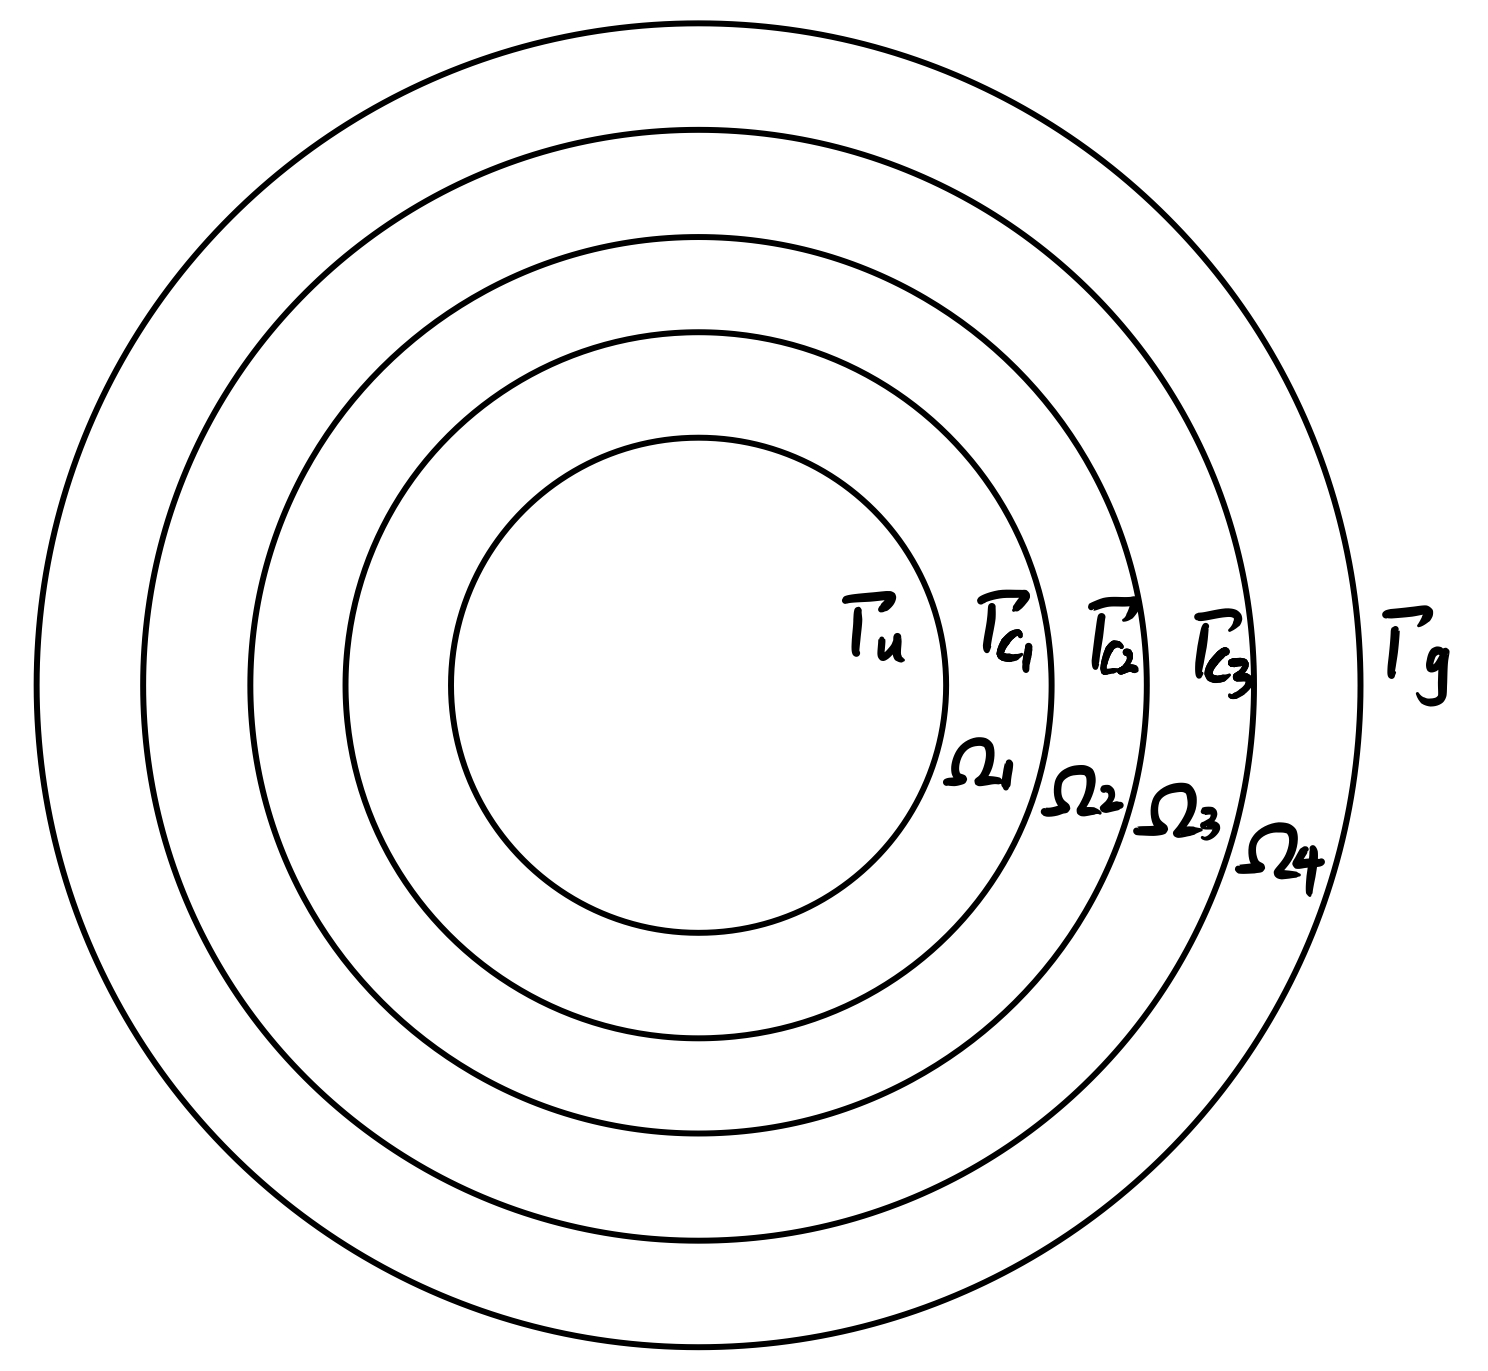
\includegraphics[scale=0.2]{fig002.png}
	\caption{domain of the multi-layers heat conduction problem}
	\label{fig001}
\end{figure}
The heat flux on boundary $\Gamma_g$ is known while it on $\Gamma_u$ is unknown. $\Gamma_{ci}(i = 1,2,\dots,N-1)$ is the interface of subdomain $\Omega_i$ and $\Omega_{i+1}$.

The primal problem is discribed as below
\begin{equation}\label{equ021}
	\left\{
	\begin{array}{lll}
		\rho_i c_i(T_i) \frac{\partial T_i}{\partial t} = \nabla \cdot \left( \lambda_i(T_i) \nabla T_i \right) \quad &(\pmb{x},t) \in (\Omega_i,\mathcal{T}) \quad &(\text{a})\\
		T_i(\pmb{x},0) = T_{i0} &\pmb{x}\in \Omega_i &(\text{b})\\
		\lambda_1(T_1) \nabla T_1 \cdot \pmb{n} = q_u(\pmb{x},t) &(\pmb{x},t)\in (\Gamma_u,\mathcal{T}) &(\text{c})\\
		\lambda_N(T_N) \nabla T_N \cdot \pmb{n} = q_g(\pmb{x},t) &(\pmb{x},t)\in (\Gamma_g,\mathcal{T}) &(\text{d})\\
		T_i(\pmb{x},t) = T_{i+1}(\pmb{x},t) &(\pmb{x},t) \in (\Gamma_i,\mathcal{T}) & (\text{e})\\
		\lambda_i(T_i) \nabla T_i \cdot \pmb{n}_i + \lambda_{i+1}(T_{i+1}) \nabla T_{i+1} \cdot \pmb{n}_{i+1} = 0 & (\pmb{x},t) \in (\Gamma_i,\mathcal{T}) & (\text{f})
	\end{array}
	\right.
\end{equation}
where $i = 1,2,\dots,N$. To inverse the unknown heat flux on boundary $\Gamma_u$. We can set sensors on boundary $\Gamma_g$ to detect the temperature distribution $Y$ on it.

\subsection{Object Function}
The object function is
\begin{equation}\label{equ022}
	\mathcal{J}(q_u) = \frac{1}{2} \int_{0}^{t_f} \int_{\Gamma_g} (T_N - Y)^2 d\Gamma dt + \frac{\gamma}{2} \int_0^{t_f} \int_{\Gamma_u} q_u^2 d\Gamma dt.
\end{equation}

Firstly, define
\begin{equation}
	\theta_i = \lim_{\epsilon \to 0} \frac{T_i(q_u + \epsilon \Delta q_u) - T_i(q_u)}{\epsilon}.
\end{equation}
So
\begin{equation}
	T_i(q_u + \epsilon \Delta q_u) \approx T_i(q_u) + \epsilon \theta_i.
\end{equation}
For simplicity, we note $T_i(q_u + \epsilon \Delta q_u)$ as $T_i^+$ and $T_i(q_u)$ as $T_i$.

Then from Eq.\ref{equ022},
\begin{align}
	\lim_{\epsilon \to 0} \frac{\mathcal{J}(q_u + \epsilon \Delta q_u) - \mathcal{J}(q_u)}{\epsilon} =& \lim_{\epsilon \to 0} \frac{1}{\epsilon} \Big[ \frac{1}{2} \int_{0}^{t_f} \int_{\Gamma_g} (T_N^+ - Y)^2 d\Gamma dt + \frac{\gamma}{2} \int_0^{t_f} \int_{\Gamma_u} (q_u + \epsilon \Delta q_u)^2 d\Gamma dt \nonumber \\
	&- \frac{1}{2} \int_{0}^{t_f} \int_{\Gamma_g} (T_N - Y)^2 d\Gamma dt - \frac{\gamma}{2} \int_0^{t_f} \int_{\Gamma_u} q_u^2 d\Gamma dt \Big] \nonumber \\
	=& \lim_{\epsilon \to 0} \frac{1}{\epsilon} \Big[ \frac{1}{2} \int_{0}^{t_f} \int_{\Gamma_g} (T_N + \epsilon \theta_N - Y)^2 d\Gamma dt + \frac{\gamma}{2} \int_0^{t_f} \int_{\Gamma_u} (q_u + \epsilon \Delta q_u)^2 d\Gamma dt \nonumber \\
	&- \frac{1}{2} \int_{0}^{t_f} \int_{\Gamma_g} (T_N - Y)^2 d\Gamma dt - \frac{\gamma}{2} \int_0^{t_f} \int_{\Gamma_u} q_u^2 d\Gamma dt \Big] \nonumber \\
	=& \lim_{\epsilon \to 0} \frac{1}{\epsilon} \Big[ \frac{1}{2} \int_{0}^{t_f} \int_{\Gamma_g} \epsilon^2 \theta_N^2 + 2\epsilon\theta_N(T_N - Y) d\Gamma dt + \frac{\gamma}{2} \int_0^{t_f} \int_{\Gamma_u} \epsilon^2 \Delta q_u^2 + 2\epsilon q_u \Delta q_u d\Gamma dt\Big] \nonumber \\
	=& \int_{0}^{t_f} \int_{\Gamma_g} \theta_N(T_N - Y) d\Gamma dt + \gamma \int_0^{t_f} \int_{\Gamma_u} q_u \Delta q_u d\Gamma dt.
\end{align}
We take the note that
\begin{equation}\label{equ023}
	(\mathcal{J}^\prime (q_u),\Delta q_u) \coloneqq \int_{0}^{t_f} \int_{\Gamma_g} \theta_N(T_N - Y) d\Gamma dt + \gamma \int_0^{t_f} \int_{\Gamma_u} q_u \Delta q_u d\Gamma dt.
\end{equation}

\subsection{Sensitivity Problem}
From Eq.\ref{equ021}(a), we have
\begin{align*}
	\rho_i c_i(T_i^+) \frac{\partial T_i^+}{\partial t} &= \nabla \cdot \left( \lambda_i(T_i^+) \nabla T_i^+ \right),\\
	\rho_i c_i(T_i) \frac{\partial T_i}{\partial t} &= \nabla \cdot \left( \lambda_i(T_i) \nabla T_i \right).
\end{align*}
Then,
\begin{align*}
	\rho_i c_i(T_i^+) \frac{\partial T_i^+}{\partial t} - \rho_i c_i(T_i) \frac{\partial T_i}{\partial t} &= \nabla \cdot \left( \lambda_i(T_i^+) \nabla T_i^+ - \lambda_i(T_i) \nabla T_i \right) \\
	\rho_i c_i(T_i^+) \frac{\partial T_i}{\partial t} + \rho_i c_i(T_i^+) \epsilon \frac{\partial \theta_i}{\partial t} - \rho_i c_i(T_i) \frac{\partial T_i}{\partial t} &= \nabla \cdot \left( \lambda_i(T_i^+) \nabla T_i + \lambda_i(T_i^+) \epsilon \nabla \theta_i - \lambda_i(T_i) \nabla T_i \right).
\end{align*}
Deviding $\epsilon$ on both sides and let $\epsilon \to 0$, we have
\begin{align}\label{equ024}
	\lim_{\epsilon \to 0}\frac{\rho_ic_i(T_i^+) - \rho_ic_i(T_i)}{\epsilon} \frac{\partial T_i}{\partial t} + \rho_i c_i(T_i^+) \frac{\partial \theta_i}{\partial t} &= \nabla \cdot \left( \lim_{\epsilon \to 0}\frac{\lambda_i(T^+_i) - \lambda_i(T_i)}{\epsilon} \nabla T_i + \lambda_i(T_i^+)\nabla\theta_i \right) \nonumber \\
	\frac{\partial \rho_i c_i(T_i)}{\partial T_i} \theta_i \frac{\partial T_i}{\partial t} + \rho_i c_i(T_i)\frac{\partial \theta_i}{\partial t} &= \nabla\cdot\left( \frac{\partial \lambda_i(T_i)}{\partial T_i} \theta_i \nabla T_i + \lambda_i(T_i) \nabla \theta_i \right) \nonumber \\
	\rho_i \frac{\partial c_i(T_i)\theta_i}{\partial t} &= \nabla \cdot \left( \nabla \lambda_i(T_i) \theta_i \right).
\end{align}

From Eq.\ref{equ021}(b), we have
\begin{equation*}
	T_i^+(t = 0) - T_i(t = 0) = T_{i0} - T_{i0}.
\end{equation*}
It is easy to get that
\begin{equation}\label{equ025}
	\theta_i(t = 0) = 0.
\end{equation}

Then, on $\Gamma_u$, based on Eq.\ref{equ021}(c)
\begin{align*}
	\left( \lambda_1(T_1^+) \nabla T_1^+ - \lambda_1(T_1) \nabla T_1 \right) \cdot \pmb{n} &= q_u + \epsilon \Delta q_u - q_u \\
	\left( \lambda_1(T_1^+) \nabla T_1 + \epsilon \lambda_1(T_1^+) \nabla \theta_1 - \lambda_1(T_1) \nabla T_1 \right) \cdot \pmb{n} &= \epsilon \Delta q_u.
\end{align*}
Deviding $\epsilon$ on both sides and let $\epsilon \to 0$
\begin{align}\label{equ026}
	\lim_{\epsilon \to 0} \left( \frac{\lambda_1(T_1^+) - \lambda_1(T_1)}{\epsilon} \nabla T_1 + \lambda_1(T_1^+) \nabla \theta_1 \right) \cdot \pmb{n} &= \delta q_u \nonumber \\
	\left( \frac{\partial \lambda_1(T_1)}{\partial T_1}\theta_1 \nabla T_1 + \lambda_1(T_1) \nabla \theta_1 \right) \cdot\pmb{n}&= \Delta q_u \nonumber \\
	\nabla \left( \lambda_1(T_1)\theta_1 \right) \cdot \pmb{n} &= \Delta q_u.
\end{align}

Similarly, we can get
\begin{equation}\label{equ027}
	\nabla \left( \lambda_N(T_N)\theta_N \right) \cdot \pmb{n} = 0
\end{equation}
on $\Gamma_g$.

Next, from Eq.\ref{equ021}(e), we can get
\begin{align}\label{equ028}
	T_i^+ - T_i &= T_{i+1}^+ - T_{i+1} \nonumber \\
	\epsilon \theta_i &= \epsilon \theta_{i+1} \nonumber\\
	\theta_i &= \theta_{i+1}
\end{align}
on $\Gamma_i$.

At last, from Eq.\ref{equ021}(f),
\begin{equation*}
	\left( \lambda_i(T_i^+)\nabla T_i^+ - \lambda_i(T_i)\nabla T_i \right) \cdot \pmb{n}_i+ \left( \lambda_{i+1}(T_{i+1}^+)\nabla T_{i+1}^+ - \lambda_{i+1}(T_{i+1})\nabla T_{i+1} \right) \cdot \pmb{n}_{i+1} = 0.
\end{equation*}
It is easy to derive that
\begin{equation}\label{equ029}
	\nabla(\lambda_i(T_i)\theta_i) \cdot \pmb{n}_i + \nabla(\lambda_{i+1}(T_{i+1})\nabla\theta_{i+1}) \cdot \pmb{n}_{i+1} = 0.
\end{equation}

Combining Eq.\ref{equ024}, Eq.\ref{equ025}, Eq.\ref{equ026}, Eq.\ref{equ027}, Eq.\ref{equ028} and Eq.\ref{equ029}, we have the sensitivity problem
\begin{equation}\label{equ030}
	\left\{
	\begin{array}{lll}
		\rho_i \frac{\partial c_i(T_i)\theta_i}{\partial t} = \nabla \cdot \left( \nabla \lambda_i(T_i) \theta_i \right) \quad &(\pmb{x},t) \in (\Omega_i,\mathcal{T}) \quad &(\text{a}) \\
		\theta_i(t = 0) = 0 & \pmb{x} \in \Omega_i &(\text{b})\\
		\nabla \left( \lambda_1(T_1)\theta_1 \right) \cdot \pmb{n} = \Delta q_u & (\pmb{x},t) \in (\Gamma_u,\mathcal{T}) &(\text{c})\\
		\nabla \left( \lambda_N(T_N)\theta_N \right) \cdot \pmb{n} = 0 & (\pmb{x},t) \in (\Gamma_g,\mathcal{T}) &(\text{d})\\
		\theta_i = \theta_{i+1} & (\pmb{x},t) \in (\Gamma_i,\mathcal{T}) &(\text{e})\\
		\nabla(\lambda_i(T_i)\theta_i) \cdot \pmb{n}_i + \nabla(\lambda_{i+1}(T_{i+1})\nabla\theta_{i+1}) \cdot \pmb{n}_{i+1} = 0 & (\pmb{x},t) \in (\Gamma_i,\mathcal{T}) &(\text{f})
	\end{array}
	\right.
\end{equation}
where $i = 1,2,\dots,N$.

\subsection{Dual Problem}
According to Eq.\ref{equ030}(a), one can get
\begin{equation*}
	0 = \sum_{i=1}^N \int_0^{t_f} \int_{\Omega_i} \left( \rho_i \frac{\partial c_i(T_i)\theta_i}{\partial t} - \nabla \cdot \left( \nabla \lambda_i(T_i) \theta_i \right) \right) \phi_i d\Omega dt.
\end{equation*}
Then,
\begin{align}
	0 =& \sum_{i=1}^N \bigg( \int_0^{t_f} \int_{\Omega_i} \rho_i \frac{\partial c_i(T_i)\theta_i}{\partial t} \phi_i d\Omega dt - \int_0^{t_f} \int_{\Omega_i} \nabla \cdot \big( \nabla \lambda_i(T_i) \theta_i \big) \phi_i d\Omega dt \bigg) \nonumber \\
	=& \sum_{i=1}^N \bigg( \int_{\Omega_i} \int_0^{t_f} \rho_i \phi_i d \big( c_i(T_i)\theta_i \big) d\Omega - \int_0^{t_f} \int_{\Omega_i} \nabla \cdot \big( \nabla \lambda_i(T_i) \theta_i \big) \phi_i d\Omega dt \bigg) \nonumber \\
	=& \sum_{i=1}^N \bigg( \int_{\Omega_i} \rho_i c_i(T_i)\theta_i \phi_i \big|_0^{t_f} d\Omega - \int_0^{t_f} \int_{\Omega_i} \rho_i c_i(T_i)\theta_i \frac{\partial \phi_i}{\partial t} d\Omega dt \nonumber \\
	&- \int_0^{t_f} \int_{\partial \Omega_i} \nabla \lambda_i(T_i) \theta_i \cdot \pmb{n} \phi_i d\Gamma dt + \int_0^{t_f} \int_{\Omega_i} \nabla \lambda_i(T_i) \theta_i \nabla \phi_i d\Omega dt \bigg) \nonumber \\
	=& \sum_{i=1}^N \bigg( \int_{\Omega_i} \rho_i c_i(T_i)\theta_i \phi_i \big|_{t_f} d\Omega - \int_0^{t_f} \int_{\Omega_i} \rho_i c_i(T_i)\theta_i \frac{\partial \phi_i}{\partial t} d\Omega dt \nonumber \\
	&- \int_0^{t_f} \int_{\partial \Omega_i} \nabla \lambda_i(T_i) \theta_i \cdot \pmb{n} \phi_i d\Gamma dt + \int_0^{t_f} \int_{\partial \Omega_i} \lambda_i(T_i) \theta_i \nabla \phi_i \cdot \pmb{n} d\Gamma dt \nonumber \\
	&- \int_0^{t_f} \int_{\Omega_i} \lambda_i(T_i) \theta_i \nabla \cdot \nabla \phi_i d\Omega dt \bigg) \nonumber 
\end{align}

\begin{align}\label{equ031}
	=& \sum_{i=1}^N \bigg( \int_{\Omega_i} \rho_i c_i(T_i)\theta_i \phi_i \big|_{t_f} d\Omega - \int_0^{t_f} \int_{\Omega_i} \Big( \rho_i c_i(T_i) \frac{\partial \phi_i}{\partial t} + \lambda_i(T_i) \nabla \cdot \nabla \phi_i \Big)  \theta_i d\Omega dt \nonumber \\
	&- \Big( \int_0^{t_f} \int_{\Gamma_g} \nabla \lambda_N(T_N) \theta_N \cdot \pmb{n} \phi_N d\Gamma dt + \int_0^{t_f} \int_{\Gamma_u} \nabla \lambda_1(T_1) \theta_1 \cdot \pmb{n} \phi_1 d\Gamma dt \nonumber \\
	&+ \int_0^{t_f} \int_{\Gamma_{i}} \nabla \lambda_i(T_i) \theta_i \cdot \pmb{n} \phi_i + \nabla \lambda_{i+1}(T_{i+1}) \theta_{i+1} \cdot \pmb{n} \phi_{i+1} d\Gamma dt \Big) \nonumber \\
	&+ \Big( \int_0^{t_f} \int_{\Gamma_g} \lambda_N(T_N) \theta_N \nabla \phi_N \cdot \pmb{n} d\Gamma dt + \int_0^{t_f} \int_{\Gamma_u} \lambda_1(T_1) \theta_1 \nabla \phi_1 \cdot \pmb{n} d\Gamma dt \nonumber \\
	&+ \int_0^{t_f} \int_{\Gamma_{i}} \lambda_i(T_i) \theta_i \nabla \phi_i \cdot \pmb{n} + \lambda_{i+1}(T_{i+1}) \theta_{i+1} \nabla \phi_{i+1} \cdot \pmb{n}d\Gamma dt\Big) \bigg) \nonumber \\
	=& \sum_{i=1}^N \bigg( \int_{\Omega_i} \rho_i c_i(T_i)\theta_i \phi_i \big|_{t_f} d\Omega - \int_0^{t_f} \int_{\Omega_i} \Big( \rho_i c_i(T_i) \frac{\partial \phi_i}{\partial t} + \lambda_i(T_i) \nabla \cdot \nabla \phi_i \Big)  \theta_i d\Omega dt \nonumber \\
	&- \Big( \int_0^{t_f} \int_{\Gamma_u} \Delta q_u \phi_1 d\Gamma dt + \int_0^{t_f} \int_{\Gamma_{i}} \nabla \lambda_i(T_i) \theta_i \cdot \pmb{n} \phi_i + \nabla \lambda_{i+1}(T_{i+1}) \theta_{i+1} \cdot \pmb{n} \phi_{i+1} d\Gamma dt \Big) \nonumber \\
	&+ \Big( \int_0^{t_f} \int_{\Gamma_g} \lambda_N(T_N) \theta_N \nabla \phi_N \cdot \pmb{n} d\Gamma dt + \int_0^{t_f} \int_{\Gamma_u} \lambda_1(T_1) \theta_1 \nabla \phi_1 \cdot \pmb{n} d\Gamma dt \nonumber \\
	&+ \int_0^{t_f} \int_{\Gamma_{i}} \lambda_i(T_i) \theta_i \nabla \phi_i \cdot \pmb{n} + \lambda_{i+1}(T_{i+1}) \theta_{i+1} \nabla \phi_{i+1} \cdot \pmb{n}d\Gamma dt\Big) \bigg).
\end{align}
On the basis of Eq.\ref{equ030}, dual problem is raised as below
\begin{equation}\label{equ032}
	\left\{
	\begin{array}{lll}
		\rho_i c_i(T_i) \frac{\partial \phi_i}{\partial t}  = - \lambda_i(T_i) \nabla \cdot \nabla \phi_i \quad &(\pmb{x},t) \in (\Omega_i, \mathcal{T}) \quad &(\text{a}) \\
		\phi_i(t = t_f) = 0 & \pmb{x} \in \Omega_i & (\text{b}) \\
		\lambda_1(T_1)\nabla\phi_1\cdot\pmb{n} = 0 & (\pmb{x},t) \in (\Gamma_u,\mathcal{T}) & (\text{c}) \\
		\lambda_N(T_N)\nabla\phi_N\cdot\pmb{n} = T_N - Y & (\pmb{x},t) \in (\Gamma_g, \mathcal{T}) & (\text{d}) \\
		\phi_i = \phi_{i+1} & (\pmb{x},t) \in (\Gamma_i,\mathcal{T}) & (\text{e}) \\
		\lambda_i(T_i)\nabla\phi_i\cdot\pmb{n}_i + \lambda_{i+1}(T_{i+1})\nabla\phi_{i+1}\cdot\pmb{n}_{i+1} = 0 & (\pmb{x},t) \in (\Gamma_i,\mathcal{T}) &(\text{f}) 
	\end{array}
	\right.
\end{equation}
where $i = 1,2,\dots,N$.

So Eq.\ref{equ031} can be written as
\begin{equation}\label{equ033}
	 0 = - \int_0^{t_f} \int_{\Gamma_u} \Delta q_u \phi_1 d\Gamma dt + \int_0^{t_f} \int_{\Gamma_g} \theta_N (T_N - Y) d\Gamma dt.
\end{equation}
Then, combine Eq.\ref{equ023} and Eq.\ref{equ033}, we can get the derivative of object function $\mathcal{J}(q_u)$ is
\begin{equation}
	\mathcal{J}^\prime (q_u) = \phi_1 + \gamma q_u.
\end{equation}

\subsection{Optimal Step Size}
Replacing $\epsilon$ with $\alpha_k$, then
\begin{align}
	\mathcal{J}(q_{u,k+1}) =& \mathcal{J}(q_{u,k} + \alpha_k \Delta q_{u,k}) \nonumber \\
	=& \frac{1}{2}\int_{0}^{t_f} \int_{\Gamma_g} (T_{N,k+1} - Y)^2 d\Gamma dt + \frac{\gamma_{k+1}}{2}\int_{0}^{t_f} \int_{\Gamma_u} (q_{u,k+1})^2 d\Gamma dt \nonumber \\
	=& \frac{1}{2}\int_{0}^{t_f} \int_{\Gamma_g} (T_{N,k} + \alpha_k \theta_{N,k} - Y)^2 d\Gamma dt + \frac{\gamma_{k+1}}{2}\int_{0}^{t_f} \int_{\Gamma_u} (q_{u,k} + \alpha_k \Delta q_{u,k})^2 d\Gamma dt \nonumber\\
	=& \frac{1}{2}\int_{0}^{t_f} \int_{\Gamma_g} (T_{N,k} - Y)^2 + \alpha_k^2 \theta_{N,k}^2 +2\alpha_k \theta_{N,k} (T_{N,k} - Y) d\Gamma dt \nonumber \\
	&+ \frac{\gamma_{k+1}}{2}\int_{0}^{t_f} \int_{\Gamma_u} q_{u,k}^2 + \alpha_k^2 \Delta q_{u,k}^2 + 2\alpha_k q_{u,k} \Delta q_{u,k} d\Gamma dt \nonumber 
\end{align}
Taking derivative of $\mathcal{J}(q_{u,k+1})$ with $\alpha_k$
\begin{equation*}
	\frac{\partial \mathcal{J}(q_{u,k+1})}{\partial \alpha_k} = \int_{0}^{t_f} \int_{\Gamma_g} \alpha_k \theta_{N,k}^2 + \theta_{N,k} (T_{N,k} - Y) d\Gamma dt + \gamma_{k+1} \int_{0}^{t_f} \int_{\Gamma_u} \alpha_k \Delta q_{u,k}^2 + q_{u,k} \Delta q_{u,k} d\Gamma dt.
\end{equation*}
Letting $\partial \mathcal{J}(q_{u,k+1}) / \partial \alpha_k$ equals to $0$, then we can get the optimal step
\begin{equation}\label{equ034}
	\alpha_k = - \frac{\int_{0}^{t_f} \int_{\Gamma_g} (T_{N,k} - Y) \theta_{N,k} d\Gamma dt + \gamma_{k+1} \int_{0}^{t_f} \int_{\Gamma_u} q_{u,k} \Delta q_{u,k} d\Gamma dt}{\int_{0}^{t_f} \int_{\Gamma_g} \theta_{N,k}^2 d\Gamma dt + \gamma_{k+1} \int_{0}^{t_f} \int_{\Gamma_u} \Delta q_{u,k}^2 d\Gamma dt}.
\end{equation}

\section{An Iterative Finite-Element Algorithm for Solving Nonlinear Inverse Heat Conduction Problems With Unknown Conduction Coefficient}

In this problem, the coefficient of heat conduction $\lambda(T)$ is unknown. Then we consider $\lambda$ is function of $\pmb{x}$ and $t$ which is $\lambda(\pmb{x}, t)$.

\subsection{Primal Problem}
\begin{equation}\label{equ001}
	\left\{
	\begin{array}{lll}
		\rho c(T) \frac{\partial T}{\partial t} = \nabla \cdot \left( \lambda \nabla T \right) \quad &(\pmb{x},t) \in (\Omega, \mathcal{T}) &\text{(a)}\\
		T(\pmb{x},0) = \tilde{Y}^\xi & \pmb{x} \in \Omega &\text{(b)}\\
		\lambda \nabla T \cdot \pmb{n} = q(\pmb{x},t) & (\pmb{x},t) \in (\partial \Omega, \mathcal{T}) &\text{(c)}
	\end{array}
	\right.
\end{equation}

\subsection{Objective Function}
From the primal problem, we define the objective function
\begin{equation}
	\mathcal{J}(\lambda) = \frac{1}{2} \int_{0}^{t_f} \int_{\partial \Omega} \left(T-Y^\xi\right)^2 d\Gamma dt + \frac{\gamma}{2} \int_{0}^{t_f}\int_{\Omega} \lambda ^2 d\Omega dt.
\end{equation}

\subsection{Sensitivity Problem}
First
\begin{equation}
	\theta (\pmb{x}, t; \lambda, \Delta \lambda) = \lim_{\epsilon \to 0} \frac{T(\pmb{x}, t; \lambda + \epsilon \Delta \lambda) - T(\pmb{x}, t; \lambda)}{\epsilon},
\end{equation}

Then 
\begin{equation}
	T(\pmb{x}, t; \lambda + \epsilon \Delta \lambda) \approx T(\pmb{x}, t; \lambda) + \epsilon \theta(\pmb{x}, t; \lambda, \Delta \lambda).
\end{equation}

Note that
\begin{align*}
	&T^+ \coloneqq T(\lambda + \epsilon \Delta \lambda),\\
	&T \coloneqq T(\lambda).
\end{align*}

From
\begin{equation}
	\rho c(T^+) \frac{\partial T^+}{\partial t} - \rho c(T) \frac{\partial T}{\partial t} = \nabla \left( (\lambda + \epsilon \Delta \lambda) \nabla T^+ \right) - \nabla \left( \lambda \nabla T \right)
\end{equation}

we can get

\begin{equation}
	\rho c(T^+) \frac{\partial T}{\partial t} - \rho c(T) \frac{\partial T}{\partial t} + \epsilon \rho c(T^+) \frac{\partial \theta}{\partial t} = \nabla \left( \epsilon \Delta \lambda \nabla T + \epsilon \lambda \nabla \theta + \epsilon^2 \Delta \lambda \nabla \theta \right)
\end{equation}

Divide $\epsilon$ on both sides of equation above and let $\epsilon$ goes to 0. We have

\begin{align}
	\lim_{\epsilon \to 0} \frac{\rho c(T^+) - \rho c(T)}{\epsilon} \frac{\partial T}{\partial t} + \rho c(T) \frac{\partial \theta}{\partial t} &= \nabla \cdot \left( \Delta \lambda \nabla T + \lambda \nabla \theta \right) \nonumber \\
	\frac{\partial \rho c(T)}{\partial T} \theta \frac{\partial T}{\partial t} + \rho c(T) \frac{\partial \theta}{\partial t} &= \nabla \cdot \left( \Delta \lambda \nabla T + \lambda \nabla \theta \right) \nonumber
\end{align}

It is easy to get

\begin{equation}
	\theta(\pmb{x}, 0) = 0.
\end{equation}

\begin{align}
	\left( \lambda + \epsilon\Delta \lambda \right) \nabla T^+ \cdot \pmb{n} &= q, \nonumber \\
	\lambda \nabla T \cdot \pmb{n} &= q.
\end{align}

\begin{align}
	\left( \epsilon \Delta \lambda \nabla T + \epsilon \lambda \nabla \theta + \epsilon^2 \Delta \lambda \nabla \theta \right) \cdot \pmb{n} &= 0 \nonumber \\		\left( \Delta \lambda \nabla T + \lambda \nabla \theta \right) \cdot \pmb{n} &= 0
\end{align}

So, the sensitivity problem is

\begin{equation}
	\left\{
	\begin{array}{lll}
		\frac{\partial \rho c(T) \theta}{\partial t} = \nabla \cdot \left( \lambda \nabla \theta + \Delta \lambda \nabla T \right)	\quad & (\pmb{x}, t) \in (\Omega , \mathcal{T}) \quad & (a) \\
		\theta (\pmb{x}, 0) = 0 \quad & \pmb{x} \in \Omega \quad & (b) \\
		\left( \lambda \nabla \theta + \Delta \lambda \nabla T \right) \cdot \pmb{n} = 0 \quad & (\pmb{x}, t) \in (\partial \Omega, \mathcal{T}) \quad & (c)
	\end{array}
	\right.
\end{equation}

\subsection{Dual Problem}
Based on the first equation of sensitivity problem
\begin{align}
	0 = & \int_{0}^{t_f} \int_{\Omega} \left[ \rho \frac{\partial c(T) \theta}{\partial t} - \nabla \cdot \left( \lambda \nabla \theta + \Delta \lambda \nabla T \right) \right] \phi d\Omega dt \nonumber \\
	= & \int_{\Omega} \rho \phi d\left( c(T) \theta \right) d\Omega - \int_{0}^{t_f}\int_{\partial \Omega} \left( \Delta \lambda \nabla T + \lambda \nabla \theta \right) \cdot \pmb{n} \phi d\Gamma dt + \int_{0}^{t_f} \int_{\Omega} \left( \Delta \lambda \nabla T + \lambda \nabla \theta \right) \nabla \phi d\Omega dt \nonumber \\
	= & \int_{\Omega} \rho \phi c(T) \theta \big|_{0}^{t_f} d\Omega - \int_{0}^{t_f} \int_{\Omega} \rho c(T) \theta \frac{\partial \phi}{\partial t} d\Omega dt + \int_{0}^{t_f} \int_{\Omega} \Delta \lambda \nabla T \nabla \phi d\Omega dt + \int_{0}^{t_f} \int_{\Omega} \lambda \nabla \theta \nabla \phi d\Omega dt \nonumber \\
	= & \int_{\Omega} \rho \phi c(T) \theta \big|_{t_f} d\Omega + \int_{0}^{t_f} \int_{\Omega} \Delta \lambda \nabla T \nabla \phi d\Omega dt + \int_{0}^{t_f} \int_{\partial \Omega} \nabla \phi \cdot \pmb{n} (\lambda \theta) d\Gamma dt - \int_{0}^{t_f} \int_{\Omega} \nabla^2 \phi \lambda \theta d\Omega dt \nonumber \\
	& - \int_{0}^{t_f} \int_{\Omega} \rho c(T) \theta \frac{\partial \phi}{\partial t} d\Omega dt \nonumber \\
	= & \int_{\Omega} \rho \phi c(T) \theta \big|_{t_f} d\Omega + \int_{0}^{t_f} \int_{\Omega} \Delta \lambda \nabla T \nabla \phi d\Omega dt + \int_{0}^{t_f} \int_{\partial \Omega} \lambda \nabla \phi \cdot \pmb{n} \theta d\Gamma dt - \int_{0}^{t_f} \int_{\Omega} \left( \rho c(T) \frac{\partial \phi}{\partial t} + \lambda \nabla^2 \phi \right) \theta d\Omega dt \nonumber
\end{align}

According to object fucntion, we can get
\begin{align}
	\mathcal{J}(\lambda + \epsilon \Delta \lambda) - \mathcal{J}(\lambda) = & \frac{1}{2} \int_{0}^{t_f} \int_{\partial \Omega} \left( T + \epsilon \theta - Y^{\xi} \right)^2 d\Gamma dt + \frac{\gamma}{2} \int_{0}^{t_f} \int_{\Omega} \left( \lambda + \epsilon \Delta \lambda \right)^2 d\Omega dt \nonumber \\
	& - \frac{1}{2} \int_{0}^{t_f}\int_{\partial \Omega} \left( T - Y^\xi \right)^2 d\Gamma dt - \frac{\gamma}{2} \int_{0}^{t_f} \int_{\Omega} \lambda^2 d\Omega dt \nonumber \\
	= & \frac{1}{2} \int_{0}^{t_f}\int_{\partial \Omega} \left( 2\epsilon \theta T - 2\epsilon \theta Y^\xi + \epsilon^2 \theta^2 \right) d\Gamma dt + \frac{\gamma}{2} \int_{0}^{t_f} \int_{\Omega} \left( 2\epsilon \lambda \Delta \lambda + \epsilon^2 \Delta \lambda^2 \right) d\Omega dt
\end{align}

Divide $\epsilon$ on both sides of the eqution above and we can get
\begin{equation}
	\lim_{\epsilon \to 0} \frac{\mathcal{J}(\lambda + \epsilon \Delta \lambda) - \mathcal{J}(\lambda)}{\epsilon} = \int_{0}^{t_f}\int_{\partial \Omega} \theta \left( T - Y^\xi \right) d\Gamma dt + \gamma \int_{0}^{t_f} \int_{\Omega} \lambda \Delta \lambda d\Omega dt
\end{equation}

So dual problem is 
\begin{equation}
	\left\{
	\begin{array}{lll}
		\rho c(T) \frac{\partial \phi}{\partial t} = - \lambda \nabla^2 \phi \quad & (\pmb{x}, t) \in (\Omega, \mathcal{T}) \quad & (a) \\
		\phi(\pmb{x}, t_f) = 0 \quad & x \in \Omega \quad & (b) \\
		\lambda \nabla \phi \cdot \pmb{n} = T - Y^\xi \quad & (\pmb{x}, t) \in (\partial \Omega, \mathcal{T}) \quad & (c)
	\end{array}
	\right.
\end{equation}

Let $\alpha_k$ represents $\epsilon$ and $p_k$ represents $\Delta \lambda$. Then we get

\begin{equation}
	\alpha_k = - \frac{\int_{0}^{t_f} \int_{\partial \Omega} \left( T_k - Y^\xi \right) \theta_k d\Gamma dt + \gamma_{k+1} \int_{0}^{t_f} \int_{\Omega} \lambda_k p_k d\Omega dt}{\int_{0}^{t_f} \int_{\partial \Omega} \theta_k^2 d\Gamma dt + \gamma_{k+1} \int_{0}^{t_f} \int_{\Omega} p_k^2 d\Omega dt}
\end{equation}

\begin{equation}
	\beta_k = 
	\left\{
	\begin{array}{l}
		0 \\
		\max(0, \beta^{PR})
	\end{array}
	\right.
\end{equation}

\begin{equation}
	\beta^{PR} = \frac{\int_{0}^{t_f} \int_{\Omega} \mathcal{J}^\prime(\lambda_k)\left[ \mathcal{J}^\prime(\lambda_k) - \mathcal{J}^\prime(\lambda_{k-1}) \right] d\Omega dt}{\int_{0}^{t_f} \int_{\Omega} \left[ \mathcal{J}^\prime(\lambda_{k-1}) \right]^2 d\Omega dt }
\end{equation}

\begin{equation}
	p_k =
	\left\{
	\begin{array}{l}
		-\mathcal{J}^\prime(\lambda_k) \\
		-\mathcal{J}^\prime(\lambda_k) + \beta_k p_{k-1}
	\end{array}
	\right.
\end{equation}

And the derivative of object function is
\begin{equation}
	\mathcal{J}^\prime(\lambda) = \nabla T \nabla \phi - \gamma \lambda
\end{equation}

\subsection{Discretization of One Dimensional Primal Problem}
\begin{equation}
	\left\{
	\begin{array}{l}
		\frac{\partial T}{\partial t} = \frac{\partial}{\partial x} \lambda \frac{\partial T}{\partial x} \\
		T(x, 0) = \tilde{Y}^\xi \\
		-\lambda \frac{\partial T}{\partial x}(0, t) = q_1(t) \\
		\lambda \frac{\partial T}{\partial x}(1, t) = q_2(t)
	\end{array}
	\right.
\end{equation}

\begin{align}
	\frac{T_{i}^{n+1} - T_{i}^n}{\Delta t} = & \frac{(\lambda_{i+1}^{n} + \lambda_{i}^{n}) T_{i+1}^{n} - (\lambda_{i+1}^{n} + 2 \lambda_{i}^{n} + \lambda_{i-1}^{n}) T_{i}^{n} + (\lambda_{i}^{n} + \lambda_{i-1}^{n}) T_{i-1}^{n}}{4 \Delta x^2} \\
	& + \frac{(\lambda_{i+1}^{n+1} + \lambda_{i}^{n+1}) T_{i+1}^{n+1} - (\lambda_{i+1}^{n+1} + 2 \lambda_{i}^{n+1} + \lambda_{i-1}^{n+1}) T_{i}^{n+1} + (\lambda_{i}^{n+1} + \lambda_{i-1}^{n+1}) T_{i-1}^{n+1}}{4 \Delta x^2}
\end{align}

\subsection{Discretization of One Dimensional Dual Problem}
\begin{equation}
	\left\{
	\begin{array}{l}
		\frac{\partial \phi}{\partial t} = - \lambda \nabla^2 \phi \\
		\phi(x, t_f) = 0 \\
		\lambda \nabla \phi \cdot \pmb{n} = T - Y^\xi
	\end{array}
	\right.
\end{equation}

It is clear that dual problem is a backward problem which has a 'final condition'. Let $t = t_f - \tau$ and we can get a forward problem.

\begin{equation}
	\left\{
	\begin{array}{l}
		\frac{\partial \phi}{\partial \tau} = \lambda \nabla^2 \phi \\
		\phi(x, 0) = 0 \\
		\lambda \nabla \phi \cdot \pmb{n} = T - Y^\xi
	\end{array}
	\right.
\end{equation}

\subsection{Discretization of One Dimensional Sensitivity Problem}

\begin{equation}
	\left\{
	\begin{array}{l}
		\frac{\partial \theta}{\partial t} = \frac{\partial}{\partial x} \left( \lambda \frac{\partial \theta}{\partial x} + \Delta \lambda \frac{\partial T}{\partial x} \right) \\
		\theta (x, 0) = 0 \\
		\lambda \frac{\partial \theta}{\partial x}(0, t) + \Delta \lambda \frac{\partial T}{\partial x}(0, t) = 0 \\
		\lambda \frac{\partial \theta}{\partial x}(1, t) + \Delta \lambda \frac{\partial T}{\partial x}(1, t) = 0 \\
	\end{array}
	\right.
\end{equation}

\subsubsection{Calcuate $\Delta \lambda$ ($p_k$)}

\begin{equation}
	p_k =
	\left\{
	\begin{array}{l}
		-\mathcal{J}^\prime(\lambda_k) \\
		-\mathcal{J}^\prime(\lambda_k) + \beta_k p_{k-1}
	\end{array}
	\right.
\end{equation}

\subsubsection{Discretization}

\begin{equation}
	\frac{\partial \theta}{\partial t} = \frac{\partial}{\partial x} \left( \lambda \frac{\partial \theta}{\partial x} + p \frac{\partial T}{\partial x} \right)
\end{equation}

\begin{align}
	\frac{\theta_{i}^{n+1} - \theta_{i}^{n}}{\Delta t} = & \frac{(\lambda_{i+1}^{n} + \lambda_{i}^{n}) \theta_{i+1}^{n} - (\lambda_{i+1}^{n} + 2 \lambda_{i}^{n} + \lambda_{i-1}^{n}) \theta_{i}^{n} + (\lambda_{i}^{n} + \lambda_{i-1}^{n}) \theta_{i-1}^{n}}{4 \Delta x^2} \nonumber \\
	& + \frac{(\lambda_{i+1}^{n+1} + \lambda_{i}^{n+1}) \theta_{i+1}^{n+1} - (\lambda_{i+1}^{n+1} + 2 \lambda_{i}^{n+1} + \lambda_{i-1}^{n+1}) \theta_{i}^{n+1} + (\lambda_{i}^{n+1} + \lambda_{i-1}^{n+1}) \theta_{i-1}^{n+1}}{4 \Delta x^2} \nonumber \\
	& + \frac{(p_{i+1}^{n} + p_{i}^{n}) T_{i+1}^{n} - (p_{i+1}^{n} + 2 p_{i}^{n} + p_{i-1}^{n}) T_{i}^{n} + (p_{i}^{n} + p_{i-1}^{n}) T_{i-1}^{n}}{4 \Delta x^2} \nonumber \\
	& + \frac{(p_{i+1}^{n+1} + p_{i}^{n+1}) T_{i+1}^{n+1} - (p_{i+1}^{n+1} + 2 p_{i}^{n+1} + p_{i-1}^{n+1}) T_{i}^{n+1} + (p_{i}^{n+1} + p_{i-1}^{n+1}) T_{i-1}^{n+1}}{4 \Delta x^2} \nonumber
\end{align}

\end{document}